
 \chapter{Sequences and Series: Commas and Plus Signs Run Amok}
 
\section{Definition of Sequences} 
\begin{definition}{Sequence}
A \emph{sequence} is a function whose domain is a subset of $\mathbb{N}=\lbrace 0,1,2,3, \ldots \rbrace $, the set of natural numbers.
\end{definition}  

Typically for $n \in \mathbb{N}$, we write $a_n$ as the output corresponding to the input $n$.  The output could technically be an object of any type, but in this course we usually use real numbers or complex numbers as our outputs.  Technically the sequence itself is the map $n \mapsto a_n$, though since this is a bit cumbersome to write, we often write just $a_n$ to refer to the entire sequence, similar to how we write $f(x)$ for a function on the real numbers. When the outputs are real numbers, we can graph sequences as a collection of points of the form (input,output) just as we would for functions on the real numbers.

\subsection{Sequences vs Functions on the Real Numbers}

The chart below compares sequences (functions whose domain is the natural numbers) and functions whose domain is the real numbers.

\begin{center}
\begin{tabular}{|l|c|c|} \hline
Trait or Notation & \bf Function on Reals & \bf Sequence  \\ \hline
 & & \\
Default Independent Variable & $x$ & $n$ \\ 
& & \\ \hline 
& & \\
Default Formula Notation & $f(x) $ & $a_n$ \\
& & \\ \hline 
& & \\
Domain $D$ & Subset of $\mathbb{R}$ & Subset of $\mathbb{N}$ \\
& & \\ \hline 
& & \\
Graph & $\left\lbrace\left(x,f(x)\right):x\in D  \right\rbrace$ & $\left\lbrace\left(n,a_n\right):n\in D  \right\rbrace$ \\
& & \\
& 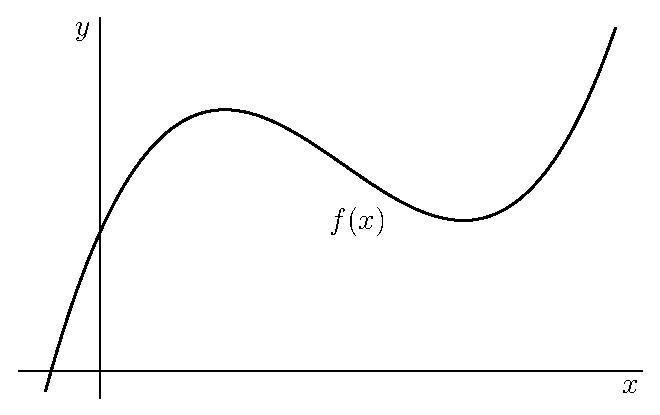
\includegraphics[width=125px]{ChapterSeqSer/Figures/SequenceGraph} & 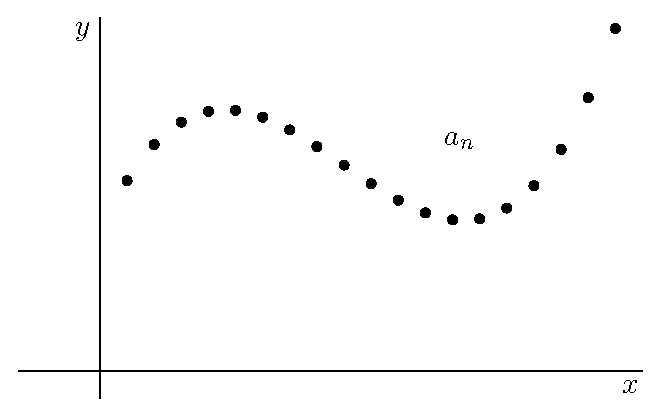
\includegraphics[width=125px]{ChapterSeqSer/Figures/SequenceGraph2} \\
\hline 
\end{tabular}
\end{center}

Less formally, a sequence is simply a \seq{list of objects}.  The correspondence between sequences as maps and sequences as lists of objects is that the $k^{th}$ object in the list is the output corresponding to $k-1$ under the map.  That is, the map $n \mapsto a_n$ corresponds to the list $a_0,a_1,a_2,a_3,\ldots$.

\begin{example}{The Sequence of Even Natural Numbers}
Consider the list of nonnegative even numbers: $0,2,4,6,8,10,\ldots$.  We can view this as the map $n \mapsto 2n $, which we can see as a function on the naturals with the following inputs and outputs:
\begin{align*}
 0 &\mapsto 0 \\
 1 &\mapsto 2 \\
 2 &\mapsto 4 \\
 3 &\mapsto 6 \\
 4 &\mapsto 8 \\
 &\vdots  \\
\end{align*}
\end{example}

\section{Notation for Sequences}

There are two main ways that we define sequences: as explicit formulas and as recursive formulas. The next two subsections describe these methods.

\subsection{Explicit Formulas}\label{exp}

Often times we define a sequence via what is called an \emph{explicit formula} or a \emph{closed formula}.  This is a formula given in terms of $n$ that shows explicitly how to compute the output corresponding to an input $n$ in finitely many steps expressed in our usual language of algebraic and transcendental functions.
\begin{example}{The Sequence of Even Natural Numbers: Explicit Formula}
The sequence of even natural numbers defined above has $$a_n=2n $$ as its \seq{explicit formula}.
\end{example}

\begin{exercise}{Practice with Explicit Formulas \Coffeecup \Coffeecup}\label{expForms}
Find an explicit formula for the sequence of...
\begin{itemize}
\item ...odd natural numbers. $$1,3,5,7,\ldots$$
\solushun{$a_n=2n+1, n\in\{0,1,2,\ldots\}$\\}{.3in}
\item ...even integers starting at -4 and counting upwards, two at a time. $$-4,-2,0,2,\ldots$$
\solushun{$-4+2n, n\in\{0,1,2,\ldots\}$\\}{.3in}
\item ...all multiples of 5, starting from 20 and counting downwards. $$20,15,10,5,0,-5,\ldots$$
\solushun{$a_n=20-5n, n\in\{0,1,2,\ldots\}$\\}{.3in}
\item ...all natural numbers that are one more than a multiple of 3. $$1,4,7,10,\ldots$$
\solushun{$a_n=3n+1,n\in\{0,1,2,\ldots\}$\\}{.3in}
\item ...consecutive powers of 2, starting from 1. $$1,2,4,8,\ldots$$
\solushun{$a_n=2^n, n\in\{0,1,2,\ldots\}$\\}{.3in}
\item ...terms that alternate forever between positive and negative one. $$1,-1,1,-1,\ldots$$
\solushun{$a_n=(-1)^n, n\in\{0,1,2,\ldots\}$\\}{.3in}
\item ...fractions whose numerators are all even natural numbers starting from zero and whose denominators are all odd natural numbers starting from 1. $$\frac{0}{1},\frac{2}{3},\frac{4}{5},\frac{6}{7},\ldots$$
\solushun{$a_n=\frac{2n}{2n+1}, n\in\{0,1,2,\ldots\}$\\}{.3in}
\end{itemize}

\end{exercise}

\subsection{Recursive Formulas}

\emph{Recursion} is a beautiful, powerful, and useful concept.  It is the idea of defining a structure in terms of smaller instances of that same type of structure.  In the case of sequences, we want to define a later term $a_n$ as a formula given in terms of $a_k$ for some $k$ values strictly less than $n$.  This definition of later terms built out of previous terms is called the \emph{recursion}.  Additionally, a recursive definition requires the definition of some initial term or terms to get the process rolling.  These early terms are called the \emph{base cases} or \emph{initial terms}.

Returning to our favorite little example once again, we ask how we can find a \seq{recursive formula} for the sequence of even numbers.  Notice how the later terms relate to the earlier terms; each term is exactly two more than the previous term.  We build a recursive formula out of this observation.

\begin{example}{The Sequence of Even Natural Numbers: Recursive Formula}

\begin{align*}
a_0 &= 0 \\
a_n &= 2 + a_{n-1}\text{ for }n \geq 1\\ 
\end{align*} 

\end{example}
\begin{exercise}{Absorbing the Language \Coffeecup}
In the recursive formula above, which expression is the base case?  Which part is the recursion? 
\solushun{$a_0=0$ is the base case and $a_n=2+a_{n-1}$ is the recursion.\\}{.2in}
\end{exercise}
\begin{exercise}{Practice with Recursive Formulas \Coffeecup \Coffeecup}
Find a recursive formula for the sequence of...
\begin{itemize}
\item ...odd natural numbers. $$1,3,5,7,\ldots$$
\solushun{$$a_0=1$$$$a_{n}=a_{n-1}+2$$}{.3in}
\item ...even integers starting at -4 and counting upwards, two at a time. $$-4,-2,0,2,\ldots$$
\solushun{$$a_0=-4$$$$a_n=a_{n-1}+2$$}{.3in}
\item ...all multiples of 5, starting from 20 and counting downwards. $$20,15,10,5,0,-5,\ldots$$
\solushun{$$a_0=20$$$$a_n=a_{n-1}-5$$}{.3in}
\item ...all natural numbers that are one more than a multiple of 3. $$1,4,7,10,\ldots$$
\solushun{$$a_0=1$$$$a_n=a_{n-1}+3$$}{.3in}
\item ...consecutive powers of 2, starting from 1. $$1,2,4,8,\ldots$$
\solushun{$$a_0=1$$$$a_n=a_{n-1}\cdot 2$$}{.3in}
\item ...terms that alternate forever between positive and negative one. $$1,-1,1,-1,\ldots$$
\solushun{$$a_0=1$$$$a_n=a_{n-1}\cdot(-1)$$}{.3in}
\item ...fractions whose numerators are all even natural numbers starting from zero and whose denominators are all odd natural numbers starting from 1. $$\frac{0}{1},\frac{2}{3},\frac{4}{5},\frac{6}{7},\ldots$$
\solushun{}{.3in}
\end{itemize}
\end{exercise}
\section{Factorials}

Some sequences have no simple explicit formula and are most easily thought of recursively.  The sequence of factorials is a famous example of this type.
\subsection{Recursive Formula for Factorials}
\begin{example}{Factorials, Defined Recursively}

Consider the following recursively defined sequence:

\begin{align*}
a_0 &= 1 \\
a_n &= n\cdot a_{n-1}\text{ for }n \geq 1\\ 
\end{align*} 

We can unwind this recursion a bit to obtain a more accessible expression for \seq{factorials}.  Observe the following calculations based on the base case and recursion given above:

\begin{align*}
a_0 &= 1 =1 \\
a_1 &= 1 \cdot a_0 = 1 \\
a_2 &= 2 \cdot a_1 = 2 \cdot 1=2 \\
a_3 &= 3 \cdot a_2 = 3 \cdot 2 \cdot 1=6 \\
a_4 &= 4 \cdot a_3 = 4 \cdot 3 \cdot 2 \cdot 1=24 \\
a_5 &= 5 \cdot a_4 = 5 \cdot 4 \cdot 3 \cdot 2 \cdot 1 = 120
\end{align*}
This sequence comes up so frequently that we give it its own symbol, the exclamation point!  Since the factorial of $n$ always amounts to the product of all natural numbers greater than or equal to 1 but less than or equal to $n$, we write the following:

$$ n! = n\cdot (n-1) \cdot (n-2) \cdots 3 \cdot 2 \cdot 1 $$

\end{example} 

Note that almost any expression involving a shady ``$\cdots$" is truthfully a recursion in disguise! 

\begin{exercise}{Why is the Factorial of Zero Equal to One? \Coffeecup}
Looking carefully at the above definition, you will notice that $$ 0!=1$$
It is a common mistake to compute 0! as 0 instead.  Here is one way to see why it should in fact be 1.

\begin{itemize}
\item If you compute $2^2$, how many numbers are you multiplying together? 

\item If you compute $2^1$, how many numbers are you multiplying together? 

\item If you compute $2^0$, how many numbers are you multiplying together?

\item Right, zero numbers are being multiplied together.  A product like this is called an \emph{empty product} and is always defined to be one, since that is the multiplicative identity.

\item If you compute 3! as the product of all natural numbers greater than or equal to 1 and but less than or equal to 3, how many numbers are you multiplying together?  

\item If you compute 2! as the product of all natural numbers greater than or equal to 1 and but less than or equal to 2, how many numbers are you multiplying together?  


\item If you compute 1! as the product of all natural numbers greater than or equal to 1 and but less than or equal to 1, how many numbers are you multiplying together?  


\item If you compute 0! as the product of all natural numbers greater than or equal to 1 and but less than or equal to 0, how many numbers are you multiplying together?  

\item Since 0! is also an empty product (much like $2^0$), what should we define it to be?
\end{itemize}
\end{exercise}
The following type of simplification will occur frequently throughout the our adventures in infinite series and power series.  They all follow directly from the recursive definition of factorials.
\begin{example}{Simplifying Factorials}
Let $n$ represent a positive natural number. Consider the expression $\frac{(n+2)!}{n!}$.  The numerator represents the product of all natural numbers between $n+2$ and 1, inclusive.  The denominator represents the product of all natural numbers between $n$ and 1, inclusive.  We expand out these products and then cancel whatever factors they have in common.
\begin{align*}
\frac{(n+2)!}{n!}&=\frac{(n+2)(n+1)(n)(n-1)(n-2)\cdots 3\cdot 2 \cdot 1}{(n)(n-1)(n-2)\cdots 3\cdot 2 \cdot 1} \\
&=(n+2)(n+1)
\end{align*}
Thus, that ratio of factorials cleans up to just a polynomial!
\end{example}
\begin{exercise}{Simplifying Factorials \Coffeecup \Coffeecup} Let $n$ be a natural number greater than or equal to 1.  Reduce the following fractions! (Are they fractorials?) \begin{itemize}
\item $\frac{n!}{(n+1)!}$
\solushun{$$\frac{1}{n+1}$$}{0in}
\item $\frac{(n+1)!}{n!}$
\solushun{$$n+1$$}{0in}
\item $\frac{(n+2)!}{n!}$
\solushun{$$(n+1)(n+1)$$}{0in}
\item $\frac{(2n+2)!}{(2n)!}$
\solushun{$$(2n+2)(2n+1)$$}{0in}
\end{itemize} \AnswerKeyEntry{\textbullet $\frac{1}{n+1}$ \textbullet $n+1$ \textbullet $(n+2)(n+1)$ \textbullet $(2n+2)(2n+1)$}
\end{exercise}
\subsection{Explicit Formula for Factorials: The Gamma Function}

The gamma function, denoted $\Gamma$, is the most common smooth interpolation of the factorial function on the positive integers.  The gamma function is \gam{defined using improper integrals}.

\begin{definition}{The Gamma Function}
For $n\in\mathbb{R}$, define
 $$ \Gamma(n)= \int_{0}^\infty x^{n-1}e^{-x}\dif x $$
\end{definition} 
That is, $\Gamma(n)$ is the area under the graph of $x^{n-1}e^{-x}$ in the first quadrant.

\begin{exercise}{Computing Values of Gamma \Coffeecup \Coffeecup \Coffeecup}
 \begin{itemize}
 \item 
 To see the manner in which the gamma function provides a continuous analog of the factorial function, fill out the values in the following table:
 
 \begin{center}
  \begin{tabular}{|| c || c | c ||}
    \hline 
    $n$ & $n!$ & $\Gamma(n)$  \\  \hline 
    1 &  &   \\ \hline
    2 &  &   \\ \hline
    3 &  &   \\ \hline
    4 &  &   \\ \hline
 \end{tabular}
\end{center}

\solushun{\begin{center}
  \begin{tabular}{|| c || c | c ||}
    \hline 
    $n$ & $n!$ & $\Gamma(n)$  \\  \hline 
    1 & 1 & 1  \\ \hline
    2 & 2 &  1 \\ \hline
    3 & 6 &  2 \\ \hline
    4 & 24 &  6 \\ \hline
 \end{tabular}
\end{center}}{0in}

 Computing the values of the gamma function will require quite a bit of work.  You don't have to show all details of the integrals above, but make sure you are comfortable doing such manipulations by hand. 
\item Given the table above, conjecture an explicit formula for the factorials.  It won't be a nice little algebraic formula, but express it in terms of an improper integral.  Write the conjecture below.

$$n!=\int_{0}^\infty \hspace*{2in} \dif x $$

\solushun{$$n!=\int_{0}^\infty x^{n}e^{-x}  \dif x$$}{0in}

\end{itemize}
\end{exercise}

Observe that you were be able to use the smaller instances of the gamma function to help you compute the larger instances!  That is, when you apply integration by parts to compute $\Gamma(n)$, it will produce an expression that involves the integral you computed for $\Gamma(n-1)$.
 
It turns out this relationship is exactly what shows that the $\Gamma$ function will \emph{always} match the values of the factorial function.  For factorial, we have:

$$ n! = n\cdot (n-1)!$$
\begin{exercise}{Gamma Recursion \Coffeecup \Coffeecup \Coffeecup}

What is the corresponding relationship for the Gamma function?  Specifically, how does $\Gamma(n)$ relate to $\Gamma(n-1)$? Write your answer below.

\solushun{
We can compute this by looking at $\Gamma(n+1)$ since it's a little easier to work with, and  computing it with integration by parts, with $u=x^n, \dif u=nx^{n-1}\dif x, v=e^{-x}, \dif v=-e^{-x}$:
\begin{align*}
    \Gamma(n+1)&=\int_0^\infty x^ne^{-x}\dif x\\
    &=\left.-x^{n}e^{-x}\right]_0^\infty+n\int x^{n-1}e^{-x}\dif x\\
    &=0+n\Gamma(n)
\end{align*}
So $\Gamma(n+1)=n\Gamma(n)$ and: $$\Gamma(n)=(n-1)\Gamma(n-1).$$
}{1in}

\end{exercise}
\subsection{An Approximation for the Factorials }\label{Stirling}

As mentioned above, there does not exist a simple algebraic \gam{explicit formula for the factorial function}.  However {\bf Stirling's Formula} gives a very nice explicit asymptotic formula.

\FormulaBox{Stirling's Formula}{\begin{tabular}{c}$ n! \sim \sqrt{2\pi n} \left( \frac{n}{e} \right)^n $\end{tabular}}

That is to say, as $n$ approaches infinity, $n!$ approaches $\sqrt{2\pi n} \left( \frac{n}{e} \right)^n$.  We don't have the tools to fully prove Stirling's Formula in this course, though it will be occasionally helpful to have a rough measure of the growth order of a factorial function.
\section{Arithmetic and Geometric Sequences}
Here we provide the \arithmeticsequence{definition}s for two particularly famous families of sequences, arithmetic and geometric.

\begin{definition}{\seq{Arithmetic} Sequence}
A sequence $a_n$ is called \emph{arithmetic} if and only if there exists some real constant $d$ such that $a_{n+1}-a_{n}=d$ for all natural numbers $n$.  In such a sequence, the number $d$ is called the \emph{common difference}.
\end{definition}

\begin{definition}{\seq{Geometric} Sequence}
A sequence $a_n$ is called \emph{geometric} if and only if there exists some real constant $r$ such that $a_{n+1}/a_{n}=r$ for all natural numbers $n$.   In such a sequence, the number $r$ is called the \emph{common ratio}.
\end{definition}

\begin{exercise}{Playing with the \geometricsequence{Definition} \Coffeecup \Coffeecup}

\begin{itemize}

\item Return to Exercise \ref{exp}.\ref{expForms}.  Which of those sequences are arithmetic?  For those that are, what is the common difference?
\solushun{
\begin{enumerate}
    \item The sequence of odd natural numbers $1,3,5,7,\ldots$ is arithmetic and has difference of $2$.
    \item The sequence of even integers $-4,-2,0,2,\ldots$ is arithmetic and has difference $2$.
    \item The sequence of multiples of $5$ is arithmetic and has difference $-5$, since the later term is less than the previous term.
    \item The sequence of natural numbers one more than a multiple of $3$, given by $1,4,7,10,\ldots$ is arithmetic and has difference of $3$.
\end{enumerate}
}{1in}


\item Return again to Exercise \ref{exp}.\ref{expForms}.  Which of those sequences are geometric?  For those that are, what is the common ratio?
\solushun{
\begin{enumerate}
    \item The sequence of consecutive powers of $2$, give by $1,2,4,8,\ldots$ is geometric, and has common ratio $2$.
    \item The sequence of alternating ones, $1,-1,1,-1,\ldots$ is geometric, with common ratio $-1$.
\end{enumerate}
}{1in}

\item Give an informal definition of an arithmetic sequence.  (Think of what you would say if you had to explain what it was to a fifth grader). 

\solushun{An arithmetic sequence grows (or decreases) by the same amount at each step. The step size from one number to the next is always the same. You add each term to the same number to get the next term.\\}{1in}

\item Give an informal definition of a geometric sequence.  (Think again of what you would say if you had to explain what it was to a fifth grader). 

\solushun{A geometric sequence grows (or shrinks) more and more at each step. You multiply each term by the same number to get the next term.\\}{1in}

\item Give an example of a sequence that is arithmetic but not geometric.
\solushun{$1.1,1.2,1.3,1.4,\ldots$.\\}{1in}

\item Give an example of a sequence that is geometric but not arithmetic.
\solushun{$1,-\frac{1}{2},\frac{1}{4},-\frac{1}{8},\cdots$.\\}{1in}

\item Can a sequence simultaneously be both arithmetic and geometric?  If it is possible, give an example of such a sequence.  If it is not possible, explain why it is not possible.
\solushun{The sequence $1,1,1,1,\ldots$ is both geometric (common ratio is $1$) and arithmetic (common difference $0$).\\}{1in}

\end{itemize}
\AnswerKeyEntry{Think about what happens if the common difference $d$ is zero and if the common ratio $r$ is 1.}
\end{exercise}

\begin{exercise}{Converting Between Recursive and Explicit Definitions \Coffeecup \Coffeecup}
\begin{itemize}

\item Write a sentence that explains the difference between defining a sequence recursively vs defining a sequence explicitly.

\solushun{Defining a sequence recursively means defining each term in relation to the previous (or several previous) terms. To find a given term, you have to calculate all the ones before it.

Defining a sequence explicitly allows us to get any term on its own.\\}{1in}

\item  Consider the following recursively-defined sequence:
\begin{align*}
 a_0&=5 \\ a_{n}&=2\cdot a_{n-1}
\end{align*}


Write out the first five terms of this sequence.  Can you find an explicit formula?

\solushun{
$$5,10,20,40,80,\ldots.$$
The explicit formula is given by $5\cdot 2^n$.\\
}{1.5in}

\item  Consider the following explicitly-defined sequence: 
$$ a_{n}=3n-2$$

Write out the first five terms of this sequence.  Can you find an recursive formula?

\solushun{\[-2,1,4,7,10,13,\ldots.\]
A recursive form is given by
$$a_0=-2$$
$$a_{n+1}=a_n+3.$$}{1.5in}

\end{itemize}
\end{exercise}
\subsection{Explicit Formulae for Arithmetic and Geometric Sequences}\label{Toemato}
\begin{example}{Explicit Formula for Arithmetic Sequences}
Since every arithmetic sequence starts with some initial term $a_0$ and then adds the same number $d$ each time to get from term to term, we can say the explicit formula will always have the same form.  In particular, we have the terms of the sequence as follows: $$a_0, a_0+d, a_0+2d, a_0+3d,\cdots. $$
Thus, a generic term of the sequence looks like $$a_n=a_0+dn$$ where $a_0$ is the initial term and $d$ is the common difference.
\end{example}
\begin{exercise}{Explicit Formula for Geometric Sequences \Coffeecup \Coffeecup}\label{UsedToBePlicit}
Repeat the process of the above example to demonstrate that every geometric sequence has explicit formula $$a_n=a_0r^n $$ where $a_0$ is the initial term and $r$ is the common ratio.

\solushun{
Since a geometric sequence starts with $a_0$ and then multiplies each term by the same common ratio, we get the sequence $$a_0,a_0\cdot r,a_0\cdot r^2,a_0\cdot r^3,\ldots.$$

Then some generic term is
$$a_n=a_0r^n.$$
}{2in}
\AnswerKeyEntry{The common ratio $r$ is what we multiply by to get from term to term.  Listing out the terms $a_0, a_0r, a_0r^2, a_0r^3,\cdots$ shows that $a_0r^n$ is the explicit formula.}
\end{exercise}